\section{Introduction to Embedded Linux}

\begin{frame}
  \frametitle{Birth of Free Software}
  \begin{columns}
    \column{0.75\textwidth}
      \begin{itemize}
      \item 1983, Richard Stallman, {\bf GNU project} and the {\bf free
          software} concept.  Beginning of the development of {\em gcc},
        {\em gdb}, {\em glibc} and other important tools
      \item 1991, Linus Torvalds, {\bf Linux kernel project}, a UNIX-like
        operating system kernel. Together with GNU software and many other
        open-source components: a completely free operating system,
        GNU/Linux
      \item ~1995, Linux is more and more popular on server systems
      \item ~2000, Linux is more and more popular on {\bf embedded
          systems}
      \item ~2008, Linux is more and more popular on mobile devices and phones
      \item ~2012, Linux is available on cheap, extensible hardware:
            Raspberry Pi, BeagleBone Black
      \end{itemize}
    \column{0.25\textwidth}
      \includegraphics[width=\textwidth]{slides/sysdev-intro/richard-stallman.jpg}
      \scriptsize
      Richard Stallman in 2019\\
      \tiny \url{https://commons.wikimedia.org/wiki/File:Richard_Stallman_at_LibrePlanet_2019.jpg}
    \end{columns}

\end{frame}

\begin{frame}
  \frametitle{Free software?}
  \begin{itemize}
  \item A program is considered {\bf free} when its license offers to
    all its users the following {\bf four} freedoms
    \begin{itemize}
    \item Freedom to run the software for any purpose
    \item Freedom to study the software and to change it
    \item Freedom to redistribute copies
    \item Freedom to distribute copies of modified versions
    \end{itemize}
  \item These freedoms are granted for both commercial and
    non-commercial use
  \item They imply the availability of source code, software can be
    modified and distributed to customers
  \item {\bf Good match for embedded systems!}
  \end{itemize}
\end{frame}

\begin{frame}{What is embedded Linux?}
  \huge
  \begin{center}
    Embedded Linux is the usage of the {\bf Linux kernel} and various
    {\bf open-source} components in embedded systems
  \end{center}
\end{frame}

\begin{frame}
  \frametitle{Advantages of Linux and Open-Source in embedded systems}
  \footnotesize
  \begin{columns}
  \column{0.5\textwidth}
     \begin{itemize}
     \item {\bf Ability to reuse components}\\
           Many features, protocols and hardware are supported.
           Allows to focus on the added value of your product.
     \item {\bf Low cost}\\
           No per-unit royalties. Development tools free
	   too. But of course deploying Linux costs time and effort.
     \item {\bf Full control}\\
           You decide when to update components in your
	   system. No vendor lock-in. This secures your investment.
     \item {\bf Easy testing of new features}\\
           No need to negotiate with third-party vendors. Just explore
	   new solutions released by the community.
     \end{itemize}
  \column{0.5\textwidth}
     \begin{itemize}
     \item {\bf Quality}\\
           Your system is built on high-quality foundations
           (kernel, compiler, C-library, base utilities...). Many
           Open-Source applications have good quality too.
     \item {\bf Security}\\
           You can trace the sources of all system components
           and perform independent vulnerability assessments.
     \item {\bf Community support}\\
           Can get very good support from the
	   community if you approach it with a constructive attitude.
     \item {\bf Participation in community work}\\
	   Possibility to collaborate with peers and get opportunities
           beyond corporate barriers.
     \end{itemize}
  \end{columns}
\end{frame}

\subsection[Systems running Linux]{A few examples of embedded systems
  running Linux}

\begin{frame}
  \frametitle{Wireless routers}
  \begin{center}
    \includegraphics[height=0.8\textheight]{slides/sysdev-intro/linksys-wireless-router.jpg}
  \end{center}
  \tiny
  Image credits: Evan Amos (\url{https://bit.ly/2JzDIkv})
\end{frame}

\begin{frame}
\frametitle{Video systems}
  \begin{center}
    \includegraphics[height=0.8\textheight]{slides/sysdev-intro/chromecast-2015.jpg}
  \end{center}
  \tiny Image credits: \url{https://bit.ly/2HbwyVq}
\end{frame}

\begin{frame}
\frametitle{Bike computers}
  \begin{center}
    \includegraphics[height=0.8\textheight]{slides/sysdev-intro/bike-computer.jpg}
  \end{center}
  \tiny
  Product from BLOKS (\url{http://bloks.de}).
  Permission to use this picture only in this document, in updates and
  in translations.
\end{frame}

\begin{frame}
\frametitle{Robots}
  \begin{center}
    \includegraphics[height=0.75\textheight]{slides/sysdev-intro/beagle-robot.jpg}
  \end{center}
  eduMIP robot (\url{https://www.ucsdrobotics.org/edumip})
\end{frame}

\begin{frame}
\frametitle{In space}
  \begin{columns}
  \column{0.5\textwidth}
  \scriptsize
  SpaceX Starlink satellites\\
  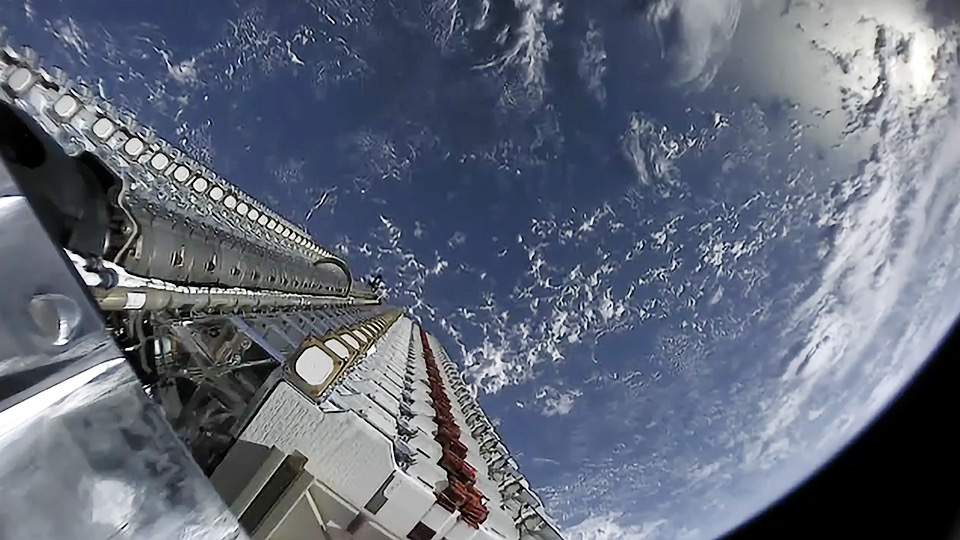
\includegraphics[height=0.3\textheight]{slides/sysdev-intro/starlink.jpg}\\
  SpaceX Falcon 9 and Falcon Heavy rockets\\
  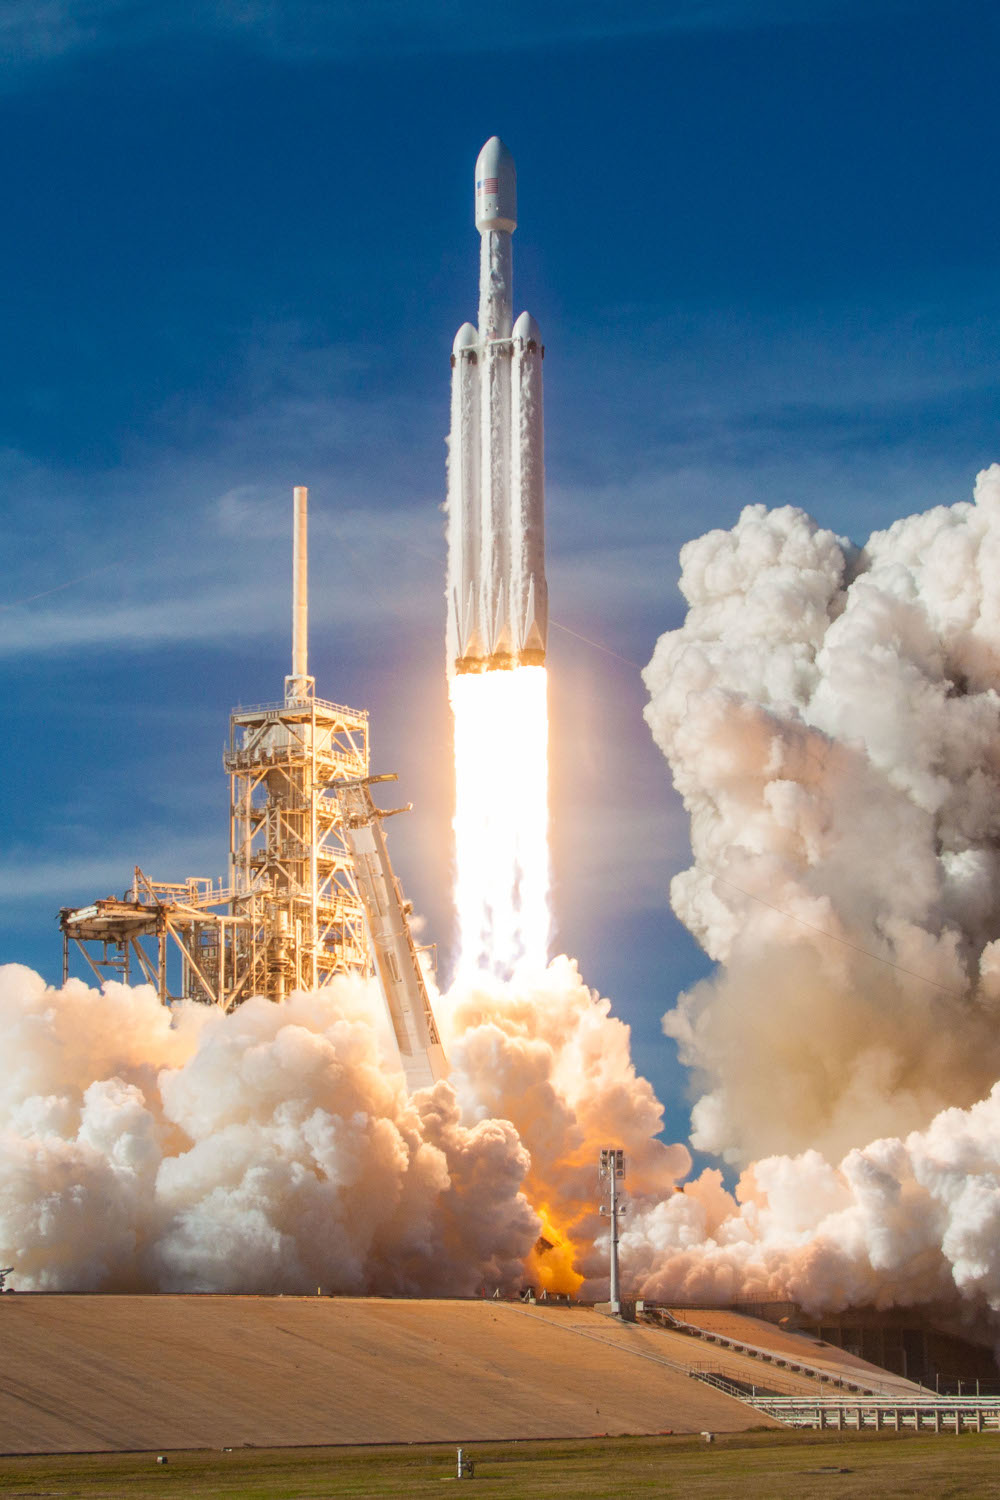
\includegraphics[height=0.3\textheight]{slides/sysdev-intro/falcon-heavy.jpg}\\
  \vspace{0.3cm}
  \tiny Image credits: Wikipedia
  \column{0.5\textwidth}
  \scriptsize
  Mars Ingenuity Helicopter\\
  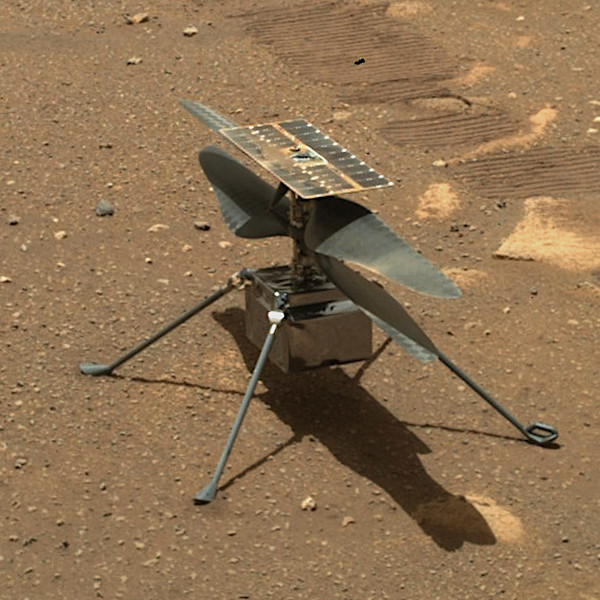
\includegraphics[height=0.3\textheight]{slides/sysdev-intro/mars-helicopter.jpg}\\
  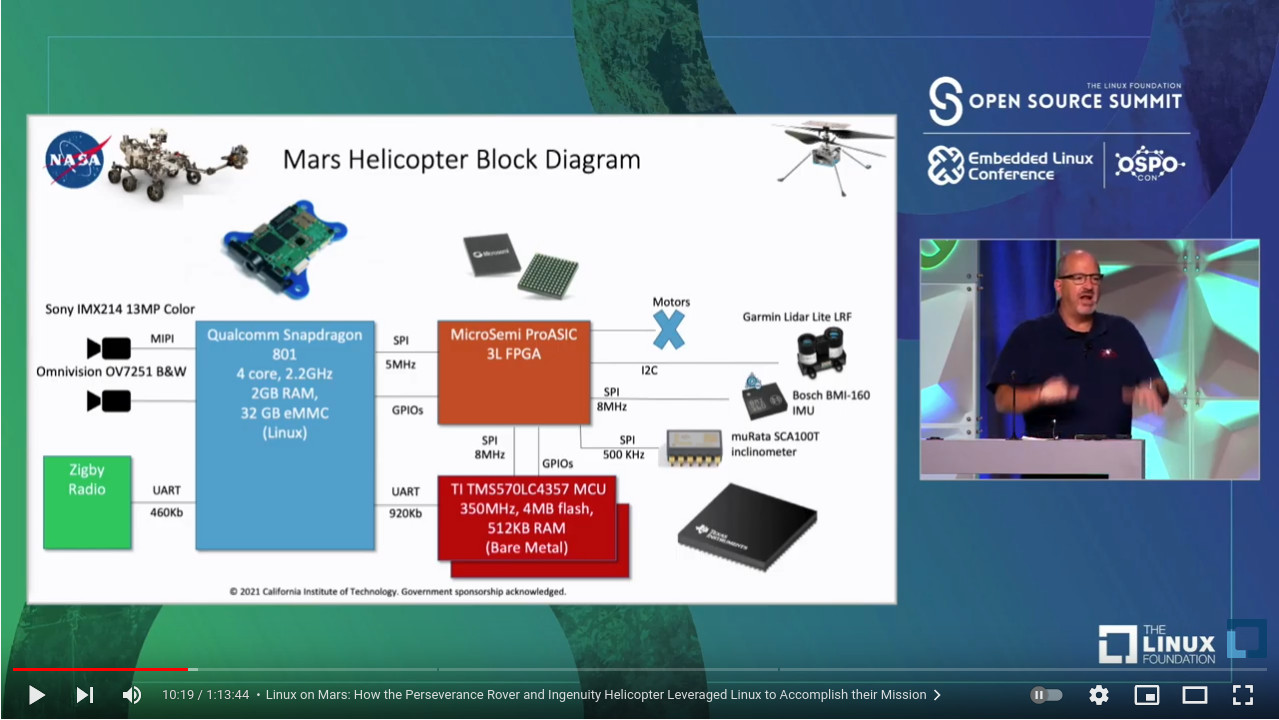
\includegraphics[height=0.3\textheight]{slides/sysdev-intro/mars-helicopter-video.jpg}\\
  \vspace{0.5cm}
  \tiny
  See the {\em Linux on Mars: How the Perseverance Rover and Ingenuity Helicopter Leveraged
  Linux to Accomplish their Mission} presentation from Tim Canham (JPL, NASA):
  \url{https://youtu.be/0_GfMcBmbCg?t=111}
  \end{columns}
\end{frame}

\subsection{Embedded hardware for Linux systems}

\begin{frame}
  \frametitle{Processor and architecture (1)}
  The Linux kernel and most other architecture-dependent
  components support a wide range of 32 and 64 bit architectures
  \begin{itemize}
  \item x86 and x86-64, as found on PC platforms, but also embedded systems
    (multimedia, industrial)
  \item ARM, with hundreds of different {\em System on Chip}s\\
        ({\em SoC}: CPU + on-chip devices, for all sorts of products)
  \item RISC-V, the rising architecture with a free instruction set\\
        (from high-end cloud computing to the smallest embedded systems)
  \item PowerPC (mainly real-time, industrial applications)
  \item MIPS (mainly networking applications)
  \item Microblaze (Xilinx), Nios II (Altera): soft cores on FPGAs
  \item Others: ARC, m68k, Xtensa, SuperH...
  \end{itemize}
\end{frame}

\begin{frame}
  \frametitle{Processor and architecture (2)}
  \begin{itemize}
  \item Both MMU and no-MMU architectures are supported, even though
    no-MMU architectures have a few limitations.
  \item Linux does not support small microcontrollers (8 or 16 bit)
  \item Besides the toolchain, the bootloader and the kernel, all
    other components are generally {\bf architecture-independent}
  \end{itemize}
\end{frame}

\begin{frame}
  \frametitle{RAM and storage}
  \begin{itemize}
  \item {\bf RAM}: a very basic Linux system can work within 8 MB of
    RAM, but a more realistic system will usually require at least 32
    MB of RAM. Depends on the type and size of applications.
  \item {\bf Storage}: a very basic Linux system can work within 4 MB
    of storage, but usually more is needed.
    \begin{itemize}
    \item {\bf Block storage}: SD/MMC/eMMC, USB mass storage, SATA, etc,
    \item {\bf Raw flash storage} is supported too, both NAND and NOR flash, with
      specific filesystems
    \end{itemize}
  \item Not necessarily interesting to be too restrictive on the
    amount of RAM/storage: having flexibility at this level allows to
    increase performance and re-use as many existing components as possible.
  \end{itemize}
\end{frame}

\begin{frame}
  \frametitle{Communication}
  \begin{itemize}
  \item The Linux kernel has support for many common communication
    buses
    \begin{itemize}
    \item I2C
    \item SPI
    \item 1-wire
    \item SDIO
    \item PCI
    \item USB
    \item CAN (mainly used in automotive)
    \end{itemize}
  \item And also extensive networking support
    \begin{itemize}
    \item Ethernet, Wifi, Bluetooth, CAN, etc.
    \item IPv4, IPv6, TCP, UDP, SCTP, DCCP, etc.
    \item Firewalling, advanced routing, multicast
    \end{itemize}
  \end{itemize}
\end{frame}

\begin{frame}
  \frametitle{Types of hardware platforms (1)}
  \begin{columns}
  \column{0.75\textwidth}
  \begin{itemize}
  \item {\bf Evaluation platforms} from the SoC vendor. Usually
    expensive, but many peripherals are built-in. Generally unsuitable
    for real products, but best for product development.
  \item {\bf System on Module} (SoM) or {\bf Component on Module}, a small
    board with only CPU/RAM/flash and a few other core components, with
    connectors to access all other peripherals. Can be used to build end
    products for small to medium quantities.
  \end{itemize}
  \column{0.25\textwidth}
    \includegraphics[width=\textwidth]{slides/sysdev-intro/stm32mp157c-ev1.png}
    \scriptsize
    STM32MP157C-EV1 evaluation board\\
    \tiny
    \href{https://www.mouser.fr/ProductDetail/STMicroelectronics/STM32MP157C-EV1?qs=9r4v7xj2LnmHBJ35TLmsRg\%3D\%3D}{Image credits}
    \vspace{0.5cm}
    \includegraphics[width=\textwidth]{slides/sysdev-intro/pocketbeagle.png}
    \scriptsize
    PocketBeagle\\
    \tiny
    Image credits (Beagleboard.org):\\
    \url{https://beagleboard.org/pocket}
  \end{columns}
\end{frame}

\begin{frame}
  \frametitle{Types of hardware platforms (2)}
  \begin{columns}
  \column{0.75\textwidth}
  \begin{itemize}
  \item {\bf Community development platforms}, to make a
    particular SoC popular and easily available. These are
    ready-to-use and low cost, but usually have fewer peripherals than
    evaluation platforms. To some extent, can also be used for real
    products.
  \item {\bf Custom platform}. Schematics for evaluation boards or
    development platforms are more and more commonly freely available,
    making it easier to develop custom platforms.
  \end{itemize}
  \column{0.25\textwidth}
    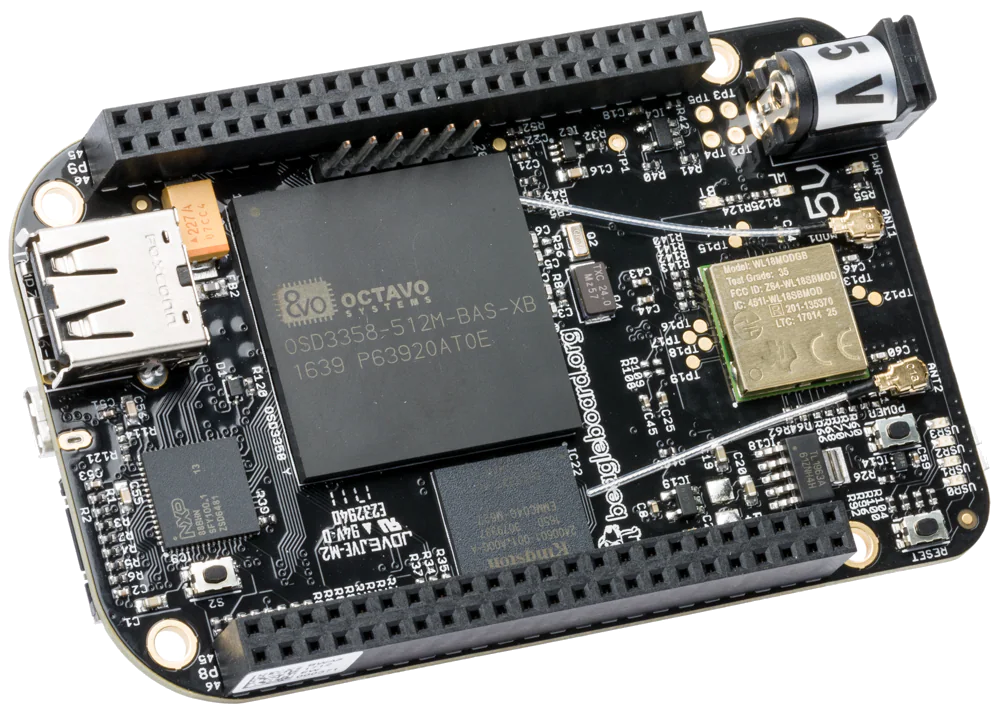
\includegraphics[height=0.3\textheight]{../slides/beagleboneblack-board/beagleboneblack.png}
    \scriptsize
    Beaglebone Black Wireless board\\
    \vspace{0.5cm}
    \includegraphics[height=0.3\textheight]{slides/sysdev-intro/teres-pcb1-a64.jpg}
    \scriptsize
    Olimex Open hardware ARM laptop main board\\
    \tiny
    Image credits (Olimex):\\
    \url{https://www.olimex.com/Products/DIY-Laptop/}
  \end{columns}
\end{frame}

\begin{frame}
  \frametitle{Criteria for choosing the hardware}
  \begin{itemize}
  \item Most SoCs are delivered with support for the Linux kernel
    and for an open-source bootloader.
  \item Having support in the official versions of the projects
    (kernel, bootloader) is a lot better: quality is better, new
    versions are available, and Long Term Support releases are
    available.
  \item Some SoC vendors and/or board vendors do not contribute their
    changes back to the mainline Linux kernel. Ask them to do so, or
    use another product if you can. A good measurement is to see the
    delta between their kernel and the official one.
  \item {\bf Between properly supported hardware in the official Linux
      kernel and poorly-supported hardware, there will be huge
      differences in development time and cost.}
  \end{itemize}
\end{frame}

\subsection{Embedded Linux system architecture}

\begin{frame}
  \frametitle{Host and target}
  \begin{center}
    \includegraphics[height=0.8\textheight]{slides/sysdev-intro/host-and-target.pdf}
  \end{center}
\end{frame}

\begin{frame}
  \frametitle{Software components}
  \begin{itemize}
  \item Cross-compilation toolchain
    \begin{itemize}
    \item Compiler that runs on the development machine, but generates
      code for the target
    \end{itemize}
  \item Bootloader
    \begin{itemize}
    \item Started by the hardware, responsible for basic
      initialization, loading and executing the kernel
    \end{itemize}
  \item Linux Kernel
    \begin{itemize}
    \item Contains the process and memory management, network stack,
      device drivers and provides services to user space applications
    \end{itemize}
  \item C library
    \begin{itemize}
    \item Of course, a library of C functions
    \item Also the interface between the kernel and the user space
      applications
    \end{itemize}
  \item Libraries and applications
    \begin{itemize}
    \item Third-party or in-house
    \end{itemize}
  \end{itemize}
\end{frame}

\begin{frame}
  \frametitle{Embedded Linux work}

  Several distinct tasks are needed when deploying embedded Linux in a
  product:

  \begin{itemize}
  \item {\bf Board Support Package development}
    \begin{itemize}
    \item A BSP contains a bootloader and kernel with the suitable
      device drivers for the targeted hardware
    \item Purpose of our \href{https://bootlin.com/training/kernel}
      {\em Kernel Development course}
    \end{itemize}
  \item {\bf System integration}
    \begin{itemize}
    \item Integrate all the components, bootloader, kernel,
      third-party libraries and applications and in-house applications
      into a working system
    \item Purpose of {\em this} course
    \end{itemize}
  \item {\bf Development of applications}
    \begin{itemize}
    \item Normal Linux applications, but using specifically chosen
      libraries
    \end{itemize}
  \end{itemize}
\end{frame}
